% =========================================================================
% Appendix F — the demiurge 7-verb pipeline (spec -> handoff). FILLED.
%   folds UFO/{spec,structure,design,analyze,synthesize,verify,handoff}/*.md:
%   per-verb deliverable fold, the verb-4 4-layer governing equations + the
%   circle-arrow fixed-point convergence, the mass budget, and a pgfplots
%   mass-budget bar chart. Honest: all landed non-wet-lab (@D d1), but
%   absorbed=false (verb-4 body-solves deferred).
% =========================================================================
\section{The demiurge 7-Verb Pipeline --- \texttt{spec} $\to$ \texttt{handoff}}
\label{app:verbs}

This appendix folds the full demiurge seven-verb design pipeline for the
integrated vehicle, all landed non-wet-lab (@D~d1). \textbf{verb-1
\texttt{spec}} defines the single-pilot payload (75\,kg, 12\,h LSS), the
7-stage matrix, and the attitude stack (gyro $\times3$, jet trim
$\times6$, EM trim, IMU $\times2$ redundancy). \textbf{verb-2
\texttt{structure}} defines the lenticular OML ($D\!=\!\SI{6}{\meter}$,
$H\!=\!\SI{1.6}{\meter}$, AR $=0.27$), the 5-bay layout, the RTSC
solenoid $\times6$ equiangular array with gyro CMG $\times3$, the 6-slot
stage mounts, and the stress budget (650\,kg, SF $=2.5$, LC-1..5).
\textbf{verb-3 \texttt{design}} gives the Stages-1--3 closed-form
parameter design (inheriting RTSC/FUSION/ANTIMATTER) and the Stages-4--7
falsifier-only mounts. \textbf{verb-4
\texttt{analyze}\,$\circlearrowleft$} specifies the 4-layer digital twin
(CFD Navier--Stokes, EM Maxwell/Meissner, structural FEA von Mises,
thermal cryo$+$radiator) with the $\circlearrowleft$ fixed-point coupling
($\max\Delta_{\text{rel}}\!<\!10^{-3}$), heavy body-solves deferred to
pool/cloud. \textbf{verb-5 \texttt{synthesize}} produces the 7-category
BOM, the L0$\to$L3 drawing tree with 7 interface drawings, and the
3-layer firmware stack (HAL / RTOS DO-178C DAL-A / app). \textbf{verb-6
\texttt{verify}} is the integrated ledger. \textbf{verb-7
\texttt{handoff}} ships the external-fab package with four certification
tracks (DO-178C, FAA Pt.25, ASME BPVC, MIL-STD-461) \emph{and the
\texttt{absorbed=false} ``not build-ready'' notice}.

% -------------------------------------------------------------------------
\subsection{Per-verb deliverable fold}
\label{app:verbs-fold}

Table~\ref{tab:verbs-detail} is the full verb roll with the landed
artifact, the concrete deliverable content, and the PR that landed it.

\begin{table}[h]
\centering
\footnotesize
\setlength{\tabcolsep}{4pt}
\begin{tabular}{@{}c l >{\raggedright\arraybackslash}m{6.0cm} c@{}}
\toprule
\textbf{\#} & \textbf{verb} & \textbf{deliverable (verbatim from \texttt{UFO/<verb>/})} & \textbf{PR} \\
\midrule
1 & \texttt{spec}       & pilot 75\,kg + 12\,h LSS; cabin $1.8{\times}1.2$\,m; 7-stage matrix; gyro$\times3$+jet$\times6$+EM trim, IMU$\times2$ & \#187 \\
2 & \texttt{structure}  & lenticular OML $D{=}6.0$\,m, $H{=}1.6$\,m, AR$=0.27$; 5-bay; RTSC solenoid$\times6$+CMG$\times3$; 6-slot mounts; 650\,kg/SF~2.5; LC-1..5 & \#190 \\
3 & \texttt{design}     & Stage-1 $NI{=}1.2{\times}10^6$\,At, $B_c{\approx}1.48$\,T; Stage-2 $B_{\text{ch}}{=}5$\,T, $F_{\text{MHD}}{\approx}9.6{\times}10^4$\,N; Stage-3 Penning $B{=}5$\,T, Ioffe 0.353\,K; Stage-4--7 falsifier-only & \#195 \\
4 & \texttt{analyze}$\circlearrowleft$ & 4-layer twin (CFD/EM/FEA/thermal) + $\circlearrowleft$ fixed point $\max\Delta_{\text{rel}}{<}10^{-3}$; heavy solves deferred (@D~d7) & pending \\
5 & \texttt{synthesize} & 7-category BOM ($\sim$32 line-items); L0$\to$L3 drawing tree; firmware HAL/RTOS(DO-178C DAL-A)/app; QA G0--G7 & --- \\
6 & \texttt{verify}     & integrated ledger \tierGreen$10$/\tierYellow$4$/\tierOrange$5$/\tierWhite$13$; Stages-1--3 nine \tierGreen; \texttt{absorbed=false} & \#206 \\
7 & \texttt{handoff}    & external-fab manifest; 4 fab competencies; 4 certification tracks (DO-178C, FAA Pt.25, ASME BPVC, MIL-STD-461); \texttt{absorbed=false} notice & --- \\
\bottomrule
\end{tabular}
\caption{The seven-verb pipeline for UFO, all landed non-wet-lab.
Implementation code is \emph{not} in these artifacts (@D~d3): all code
SSOT lives under hexa-lang \texttt{stdlib/}; the \texttt{UFO/<verb>/}
files are docs/manifests only. ``Landed'' means the non-wet-lab artifact
is complete (@D~d1), \emph{not} that the vehicle is built or flown.}
\label{tab:verbs-detail}
\end{table}

% -------------------------------------------------------------------------
\subsection{The verb-4 4-layer digital twin and the $\circlearrowleft$ coupling}
\label{app:verbs-analyze}

The \texttt{analyze}\,$\circlearrowleft$ verb is the iterative core. It
couples four physics layers, each with its own governing equation, into a
fixed-point loop (Table~\ref{tab:verbs-layers}):

\begin{table}[h]
\centering
\small
\setlength{\tabcolsep}{4pt}
\begin{tabular}{@{}c l l >{\raggedright\arraybackslash}m{4.2cm}@{}}
\toprule
\textbf{layer} & \textbf{physics} & \textbf{governing equation} & \textbf{key output / cited atom} \\
\midrule
\textcircled{\scriptsize 1} & CFD & compressible Navier--Stokes (RANS k-$\omega$ SST $\to$ DES) & $C_d$, $L/D$, $F_{\text{drag}}$ (Mach 0.5--25) \\
\textcircled{\scriptsize 2} & EM & Maxwell--Amp\`ere + Meissner & $B$-map, $F_{\text{lift}}$, $F_{\text{MHD}}{=}J{\times}B$; \texttt{ioffe\_loop\_bz} \tierGreen\ $\times3$ \\
\textcircled{\scriptsize 3} & FEA & linear-elastic, von Mises & $\sigma_v\!\le\!\sigma_{\text{allow}}$, SF (LC-1..5) \\
\textcircled{\scriptsize 4} & thermal & $k\nabla^2T=\rho c\dot T$, $\dot Q=\varepsilon\sigma_{\text{SB}}T^4$ & heat leak, radiator $A$, cryo stability \\
$\circlearrowleft$ & coupling & fixed-point iteration & $\max(\Delta_{\text{rel}})<10^{-3}$ across all 4 \\
\bottomrule
\end{tabular}
\caption{The verb-4 4-layer twin
(\texttt{UFO/analyze/integrated-vehicle-analyze.md}). The Lorentz body
force $F_{\text{body}}=J\times B$ couples EM into the CFD momentum
equation; EM ohmic heat $q'''$ couples into the thermal layer; the
thermal field feeds back $T$-dependent $\rho,\sigma_e,B_c$. The loop
converges when the relative change across all four layers drops below
$10^{-3}$. The heavy body-solves (3-D compressible CFD, 6-coil 3-D FEM,
explicit-dynamic FEA, transient cryo) are \tierOrange\ deferred to
pool/cloud (@D~d7); only the closed-form anchors and the convergence
criterion are closed in this verb (\S\ref{app:gateinv}).}
\label{tab:verbs-layers}
\end{table}

% -------------------------------------------------------------------------
\subsection{The mass budget}
\label{app:verbs-mass}

The verb-2/3 mass budget closes the 650\,kg craft at SF $=2.5$
(Fig.~\ref{fig:verbs-mass}): magnet array 120\,kg, power/stage modules
150\,kg, CFRP frame 180\,kg, life-support 80\,kg, and pilot payload
120\,kg (pilot + seat + consumables). The structural FEA (LC-1..5)
returns $\sigma_{v,\max}=0.771$--$9.254$\,MPa against
$\sigma_{\text{allow}}=600$\,MPa (T700 CFRP quasi-isotropic), i.e.\
SF $\ge\!64.8\gg2.5$ --- a natural consequence of a light disc under
inertial load, not a forced number (@D~d6).

\begin{figure}[h]
\centering
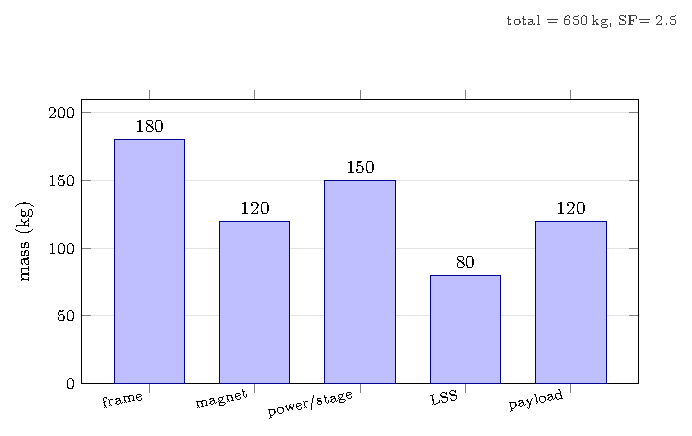
\includegraphics[width=0.78\linewidth]{figures/fig08_mass_budget.pdf}
\caption{The UFO mass budget (650\,kg total, verb-2 structure \S5).
Five categories --- frame (CFRP), magnet array (RTSC solenoid$\times6$ +
cryostat), power/stage modules (Stage-1--3), life-support (12\,h LSS),
and pilot payload --- sum to 650\,kg at SF~$=2.5$. The structural FEA
finds these loads give SF~$\ge\!64.8$ against the CFRP allowable, so the
craft is mass-light, not stress-limited. The Stage-4--7 mounts add no
mass (formal slots only).}
\label{fig:verbs-mass}
\end{figure}

% -------------------------------------------------------------------------
\subsection{Honest scope --- complete but not build-ready}
\label{app:verbs-scope}

Every verb has a landed non-wet-lab artifact (@D~d1), so the pipeline is
\emph{complete} in the demiurge sense. It is \emph{not} build-ready: the
verb-6 \texttt{verify} ledger pins the heavy verb-4 body-solves as
\tierOrange\ deferred and the Stage-4--7 falsifiers as \tierWhite\ open,
and the verb-7 \texttt{handoff} package carries an explicit
\texttt{absorbed=false} ``not production-ready'' notice. ``Pipeline
complete'' and ``vehicle build-ready'' are different claims; UFO makes
the first and explicitly disavows the second.
